\documentclass[tikz,border=10pt]{standalone}
\usepackage{tikz}
\usepackage{fontawesome6}
\usetikzlibrary{arrows.meta}
\usetikzlibrary{decorations.pathreplacing}
\usepackage[dvipsnames]{xcolor}
\usetikzlibrary{trees}
\begin{document}
\begin{tikzpicture}[scale=1.6,
    every node/.style = {draw=black, thick, anchor=west},
    selected/.style = {draw=OliveGreen, fill=green!30},
    file/.style = {draw=blue, fill=cyan!30},
    optional/.style = {dashed, fill=gray!50},
    grow via three points={one child at (0.5,-0.7) and two children at (0.5,-0.7) and (0.5,-1.4)},
    edge from parent path={(\tikzparentnode.south) |- (\tikzchildnode.west)}
]
\node [selected] {\faFolder[regular] /User}
child { 
    node [selected] {\faFolder[regular] /Cours}
    child { 
        node [selected] {\faFolder[regular] /Cours\_1}
        child { 
            node [file] {\faFile[regular] Slides\_1.pdf}
        }
    }
}
child [missing] {}
child [missing] {}
child { 
    node [selected] {\faFolder[regular] /TPs}
    child { 
        node [selected] {\faFolder[regular] /Solutions}
    }
    child { 
        node [file] {\faFile[regular] tp1.py}
    }
    child { 
        node [file] {\faFile[regular] tp1.java}
    }
}
child [missing] {}
child [missing] {}
child [missing] {}
child { 
    node [selected] {\faFolder[regular] /Documents}
}
child { 
    node [selected] {\faFolder[regular] /Photos}
};
\end{tikzpicture}
\end{document}